%
%  revised  introduction.tex  2011-09-02  Mark Senn  http://engineering.purdue.edu/~mark
%  created  introduction.tex  2002-06-03  Mark Senn  http://engineering.purdue.edu/~mark
%
%  This is the introduction chapter for a simple, example thesis.
%


\chapter{INTRODUCTION}

Since the nineteenth century, machines have been playing more and more important roles in every aspect all around the world. Especially in modern factories, a few workers with a well-designed mechanical production line are capable to accomplish the job that used to require hundreds of skilled workers to do. Specifically, machines brought to us not just efficiency, but also accuracy and reliability. Therefore, automatizing production or, rather, replacing human workers with robots is imperative for every production plant.


\section{Introduction to Indoor AGVs and Their Guidance Systems}

In the 1950s, the first Automatic Guided Vehicle (AGV) a tow truck following a wire in the floor was introduced by Barrett Electronics to handle materials for a production line. \cite{olmi2011traffic} However, after decades of development, AGVs are able to help achieve the unmanned production line in many factories. Modern AGVs with built-in microprocessors can be controlled by computer. Therefore they are not only able to move heavy materials around, but they are also significantly accurate and reliable. A typical AGV can have over $1,000$ pounds of load capacity; in addition, the tracking accuracy is just $\pm 1.27 cm$. \cite{KESH} 
		
There are many types of AGVs, such as towing vehicles, unit load carriers, forklift trucks, and so on. They all move around factories by following guidance systems.  
		
%\section{Current AGVs}
The most popular guidance systems for current indoor AGVs are wire-guided, optical, inertial, infrared, laser, and teaching type. \cite{KESH}

\begin{itemize}
    \item Wire-Guided:
    \begin{itemize}
    \item An energized wire is rooted along the guide path. 
    \item The antenna of the AGV follows the rooted wire.
    \end{itemize}
    %The outdoor crop field is very large compared to the indoor factories. It is too expensive to root wire under ground in advance. And because of the variety of the temperature and humidity, the wire is easy to be eroded.
    \item Optical:
    \begin{itemize}
    \item Colorless fluorescent particles are painted on the concrete/tiled floor. 
    \item Photosensors are used to track these particles.
    \end{itemize}
    %It is impossible to paint the colorless florescent particles on the soil.
    \item Inertial:
    \begin{itemize}
    \item The guide path is programmed on a microprocessor that is fixed on the AGV. 
    \item A sonar system is incorporated for finding obstacles.
    \end{itemize}
    %Sonar system cannot be used as a guide system in an open area.
    \item Infrared:
    \begin{itemize}
    \item Infrared light transmitters are used to detect the position of the vehicle.
    \item Reflectors are affixed on the top of the vehicle to reflect the light.
    \end{itemize}
    %It is hard to detect the position of the vehicle by using infrared light transmitters in under sunlight.
    \item Laser:
    \begin{itemize}
    \item A laser beam is used to scan wall-mounted bar-coded reflectors.
    \item Accurate positioning can be obtained.
    \end{itemize}
    %This is using for a very close distance to enhance accuracy.
    \item Teaching type:
    \begin{itemize}
    \item The AGV learns the guide path by moving along the required route.
    \item The AGV sends the information to the host computer.
    \end{itemize}
    %The outdoor ground is rough and unpredictable. It is hard to stay in the planned route by just memorizing it. Because small errors of moving on rough ground cumulates to big errors. 
\end{itemize}
%It is obvious that none of the indoor AGVs guide systems are suitable for outdoor AGVs.

In general, the guide could be pre-rooted wire, magnet, or colorless florescent particles of paint. All of these AGVs are fairly accurate, but they can only work indoors. Wires and magnets need to be planted underground, and paint needs to be painted on concrete or tiled floor. The indoor environment can be well controlled, while an outdoor environment cannot because it is very complicated and unpredictable. The ground could be rugged, wet, or steep, and because the terrain is exposed, it is susceptible to cold or rain, as well as dust, light, and the Earth's magnetic field. This paper will provide a solution to bring AGVs from indoor to outdoor use, and introduce AGV to the field of precision agriculture.

\section{Introduction to Outdoor Farm Machinery and Their Guidance Systems}

%引入介绍农业机械的导航系统
For thousands of years, farming has been one of the most important methods to harvest food. There has been a big leap from traditional farming, where the farmer could only get help from cattle or horses, to modern farming, where the farmer could get help from farm machinery. It is possible to satisfy the explosive food demand of the world's human population because of the development of farming technology.

Combine harvesters are one of the most famous farm machinery. They are well-known for their efficiency and convenience. The traditional procedure of harvesting wheat is cutting, sheaving, drying, threshing, and winnowing. On a modern farm, the whole process can be done by a combine harvester, which is a big leap forward for harvesting crops. However, modern farming is not only about harvesting; it is also about tilling, seeding, watering, fertilizing, and so on. And all the rest of this work is done by tractors and appropriate attachments.
\begin{figure}[ht!]
\begin{center}
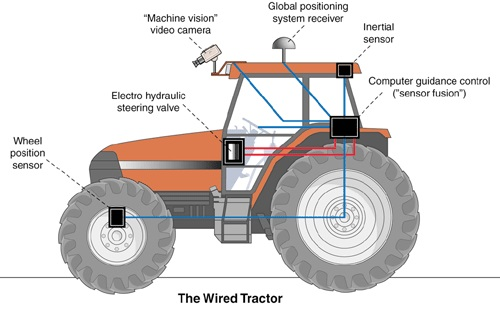
\includegraphics[scale = 1]{pics/GPStractor.jpg}
\caption{Tractor With GPS Guidance System}
\end{center}
\end{figure}

Tractor is the core machine of field work. It can do different jobs with different attachments. Figure  1.1 shows a modern tractor with many sensors installed. The most significant one is the GPS receiver. The GPS guidance system is one of the most popular guidance systems that works outdoors. Under the help of a GPS guidance system, the field usage efficiency can be optimized. However, the accuracy of GPS is always a problem. Although there is a improved solution for GPS, which has brought the accuracy to centimeter level, the cost becomes very expensive.

\section{Importance of Subject}

Labor is one of the most significant factors of agriculture. With the help of farm machinery, the total amount of labor dedicated to farming has decreased by about 30 percent for hired labor and about 40 percent for self-employed labor from 1982 to 2007. Moreover, the farm output increased by 35 percent (Table 1.1) while the total amount of labor dedicated to farming was decreased. \cite{o2011changing} %So the machines are really good helpers to farm. 
\begin{table}[ht!]
\begin{center}
\caption{The Change Labor and Output in Agriculture}
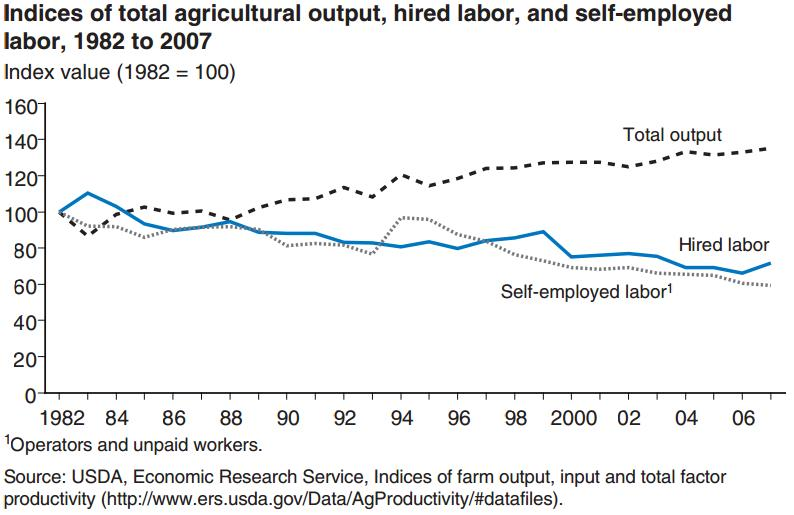
\includegraphics[scale = 0.7]{pics/laborandoutput.jpg}
\end{center}
\end{table}
Undoubtedly, the usage of farm machinery not only lowers the amount of labor, but also increases the productivity. 

In late 20th century, Pierre Robert proposed, developed, and popularized precision agriculture. \cite{mcbratney2005future} Most of the farm machinery now has the GPS, which stands for Global Positioning System, on board because of his contribution. It is very easy to plant all crops in nicely columns with the GPS guidance system. GPS-mounted farm machinery did a great job in the past few years, but there is a problem. The accuracy of the original GPS is typically about a few meters. Fortunately, technology improved the accuracy to $\pm$ 10 $cm$. \cite{thuilot2002automatic} Although this $\pm$ 10 $cm$ accuracy is acceptable with most popular 76.2 $cm$ row spacing, not for 50.8 $cm$ or 38.1 $cm$ row spacings that will be used in the future. \cite{fawcett2014farm} And the experiment field has an even higher requirement. The objective of the experiment field is to find the highest quality breed of crops. Therefore, it is extremely important to keep the growth environment of every plant at the same level, and the position to seed the experiment field is strict. Every plant should be kept at the same distance to one other, which is the precondition to provide every plant the same amount of water, sunlight, fertilizer, and carbon dioxide. Failure to do this will cause the result of the experiment to be meaningless. As a result, it is vital to have outdoor AGVs working as accurately as the indoor ones.

\section{Knowledge Gap}

Currently in the United States, the products of modern farming not only fulfill food demand of the United States, but also surpass it. For example, more than 70 percent of the volume of U.S. production of Cotton and Tree nuts were exported from 2011 to 2013 (Table 1.2). And the overall average annual export share of U.S. agricultural production is 20 percent since 2000. \cite{Exports}
\begin{table}[ht!]
\begin{center}
\caption{Export Share of U.S. Farm Production, 2011-13}
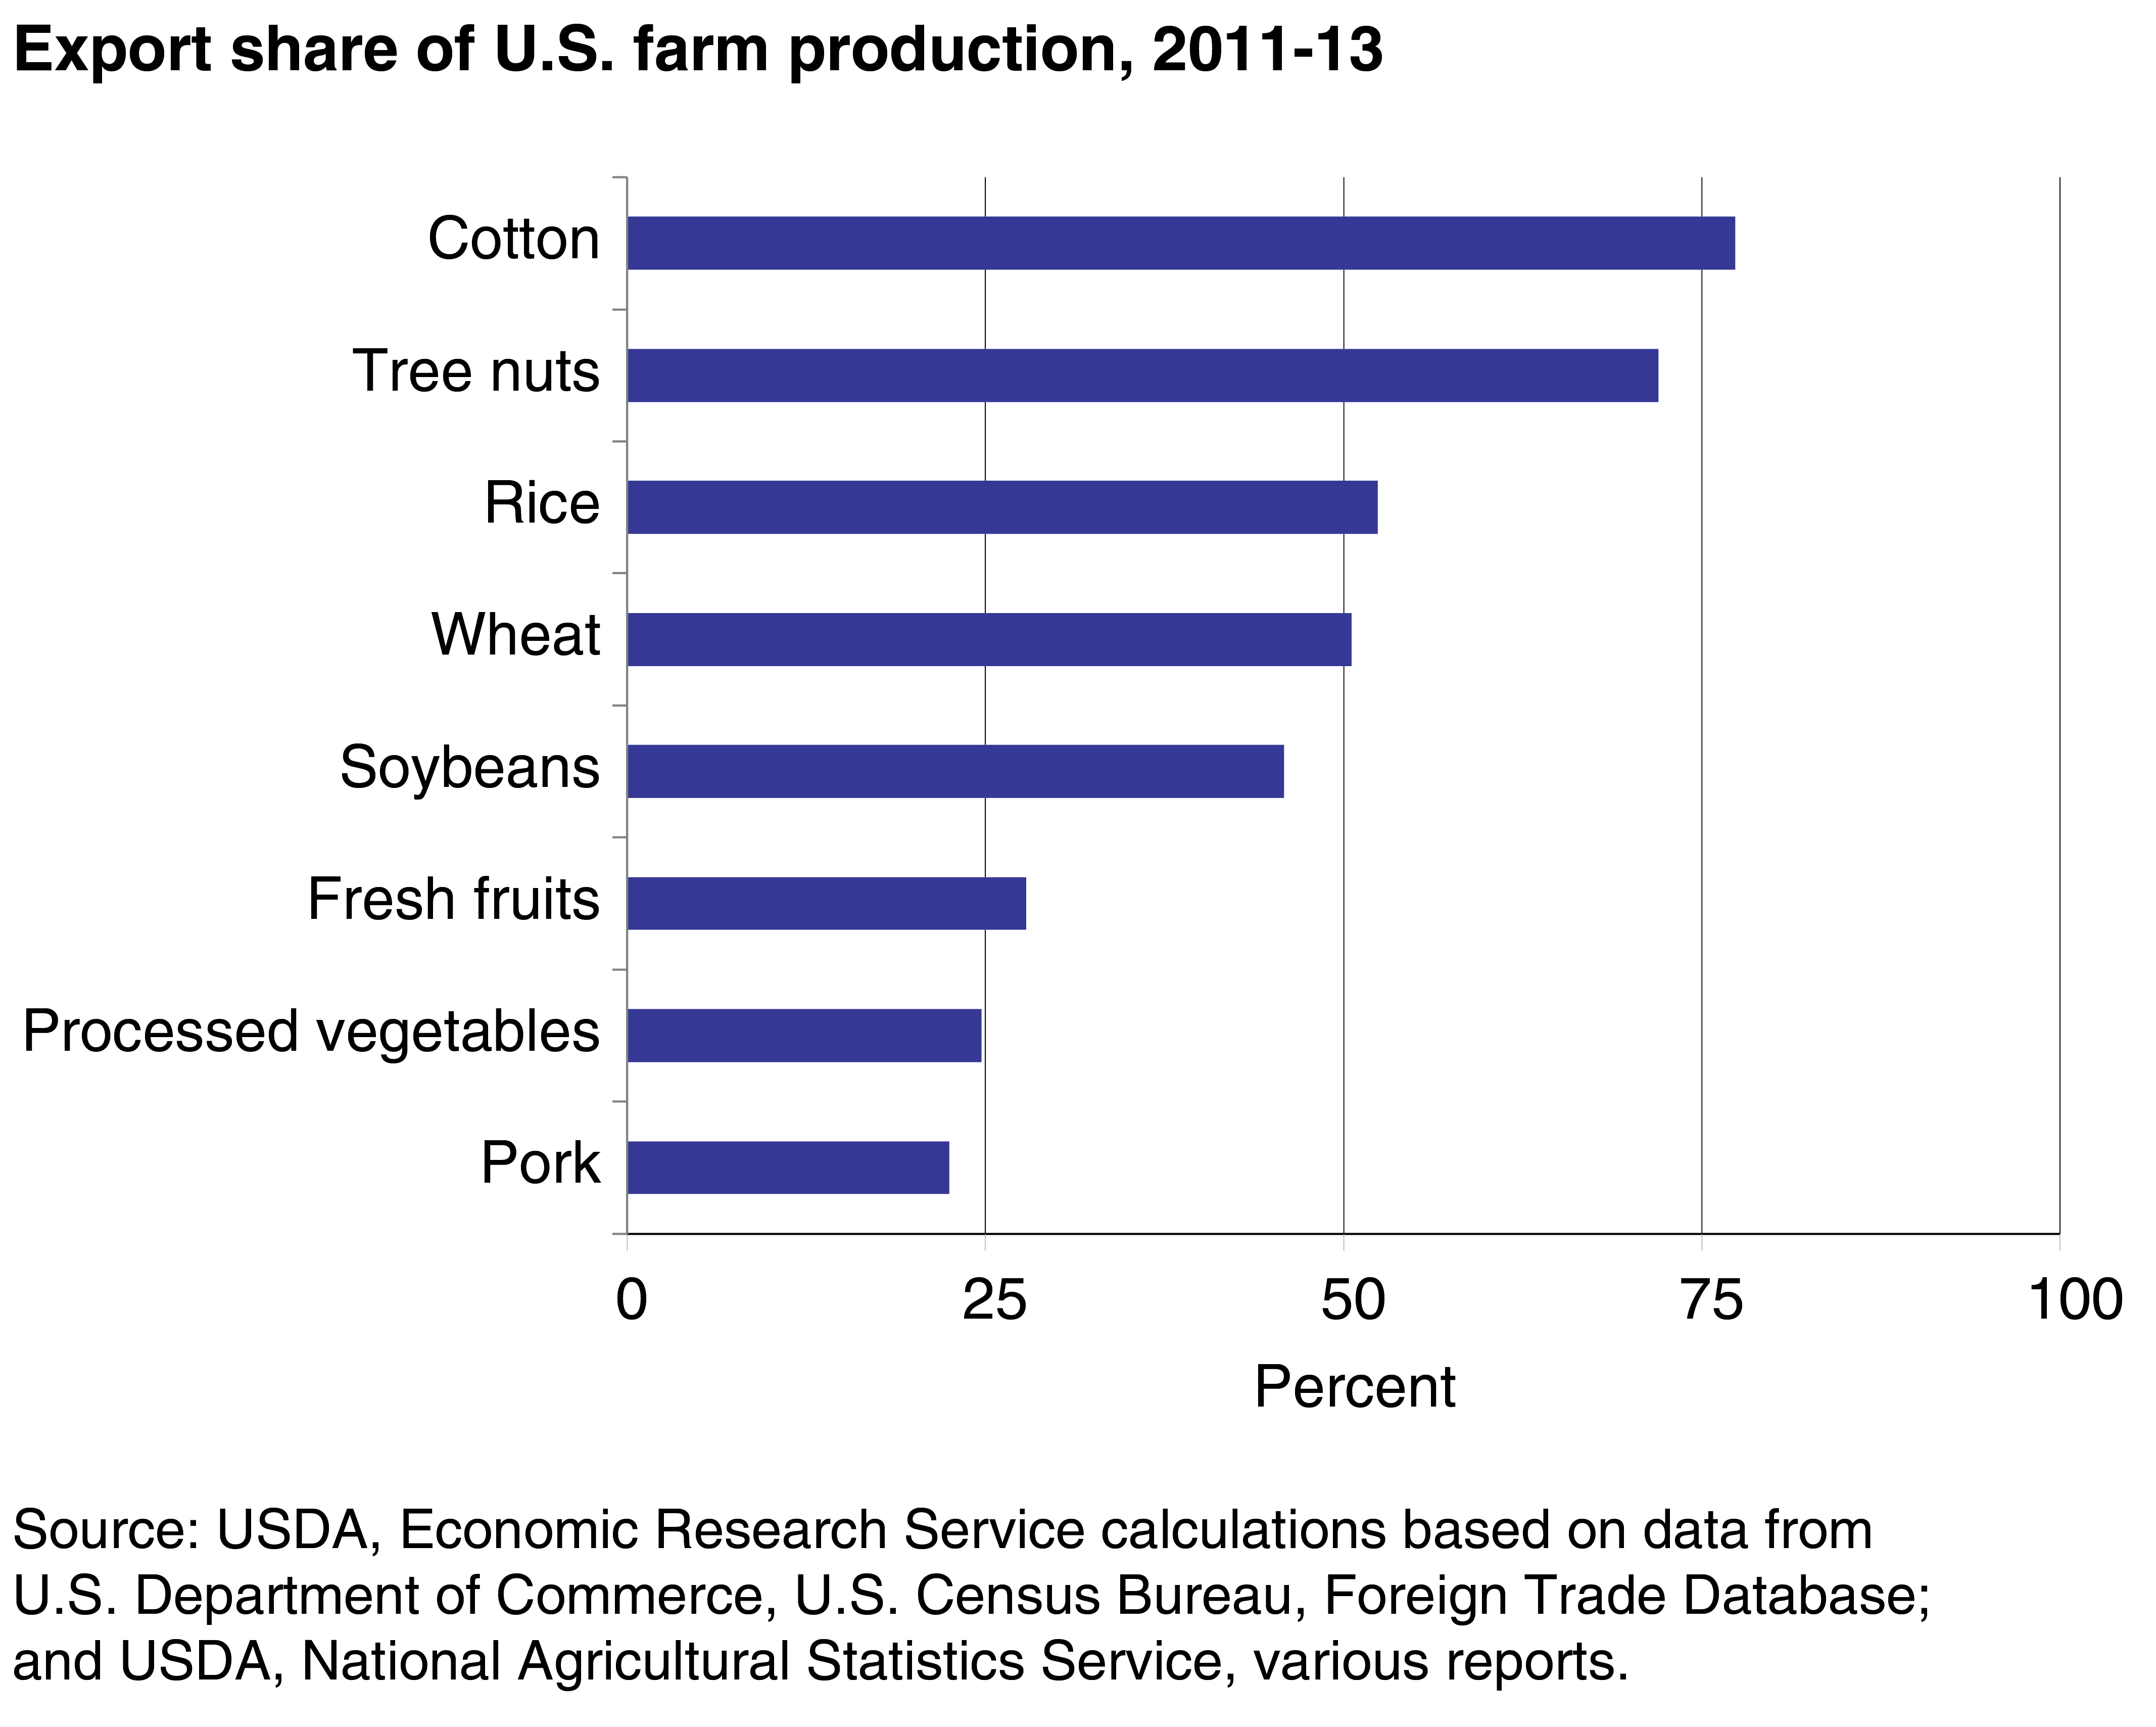
\includegraphics[scale = 0.4]{pics/cropexport.png}
\end{center}
\end{table}
Since there is no food shortage in the United States, the technology of farm machinery seems to be more than enough. However, there are many other places in the world where it is very hard to grow crops, because the farming conditions are totally different compared to North America. 
\subsection{Situations Which Require Higher Accuracy}
The water scarcity in West Asia and North Africa is a well-known problem. The world average annual per capita renewable supplies of water was about $7000 m^{3}$ in 1999; however, it was below $1500 m^{3}$ in West Asia and North Africa at the same time. More seriously, this level was $3500 m^{3}$ in 1960, and it was expected to continuously decrease to less $700 m^{3}$ by the year of 2025. \cite{margat1999water} One of the best solutions for water scarcity is to use micro-irrigation, or more specifically, drip irrigation (Figure 1.2). 
\begin{figure}[ht!]
\begin{center}
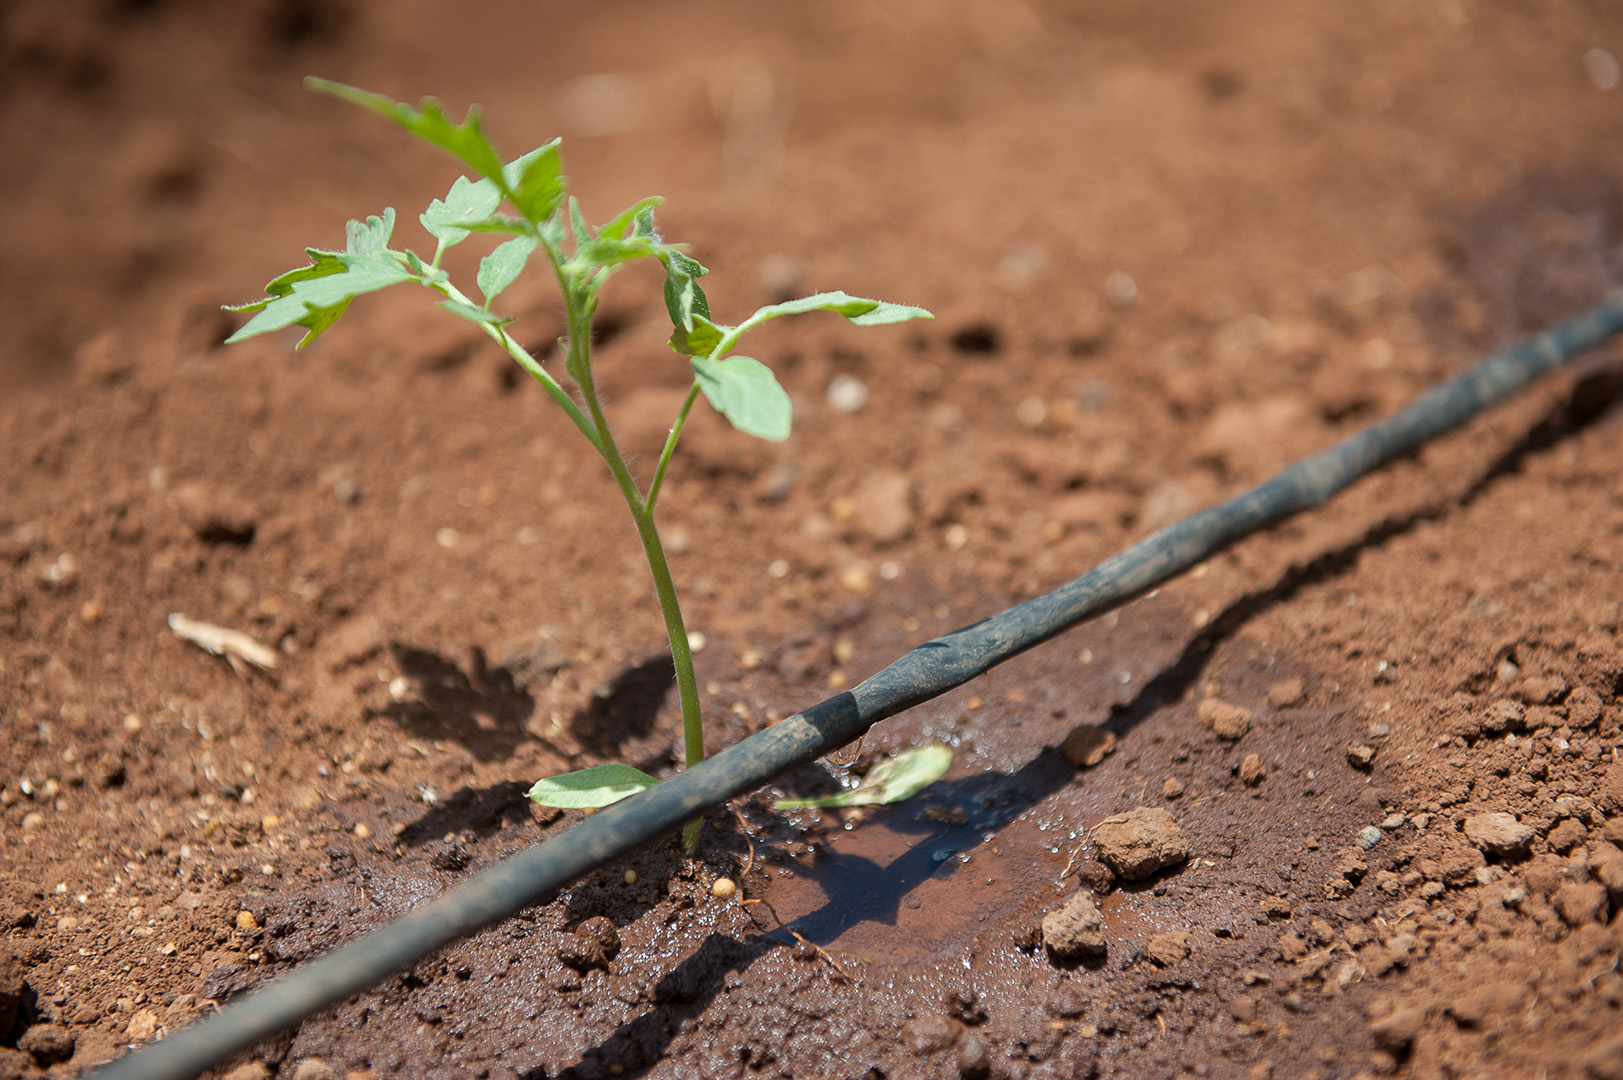
\includegraphics[scale = 0.2]{pics/drip.jpg}
\caption{Drip Irrigation}
\end{center}
\end{figure}
Some advantages of micro-irrigation include improved water and nutrient management, potential for improved yields and crop quality, greater control of applied water resulting in less water and nutrient loss through deep percolation, and reduced total water requirements. \cite{phene1986advantages} Unfortunately, the applications of micro-irrigation is also limited. Mostly, micro-irrigation is used on permanent plantings such as trees and vines. The reason that it is not used on the field crops is that it needs to be installed and removed at the beginning and the end of each growing season. Furthermore, field corps are different from trees and vines; their height is low, so the working zone is close to the ground. Therefore, the drip tubes make the other fields operations more difficult than it used to be. An improved method to make it possible to use micro-irrigation on field corps is to bury the tubes underground. \cite{camp1998subsurface} Although the tubes neither affect the field operations nor need to be reinstalled every growing season, the position of the drip spot is fixed once it is buried. So the problem turns into planting crops in the right position, which can be solved by the outdoor AGV that this paper introduces. 

\subsection{Situations Which Require Lower Cost}

The development of China is not comprehensive, and farming especially is not developed. Table 1.3 show the difference of cereals productivity between China and the United States. The cereals productivity of China is only 75.4\% compare to the United States. However, the labor dedicated for agriculture is about 300 million in China, while this number is only about 2 million in the United States. The disparity in this number shows that the per capita arable land is only about $0.3 hm^{2}$ in China, while it is about $61 hm^{2}$ in the United States. \cite{tao2012}
\begin{table}[ht!]
\begin{center}
\caption{Cereals Productivity}
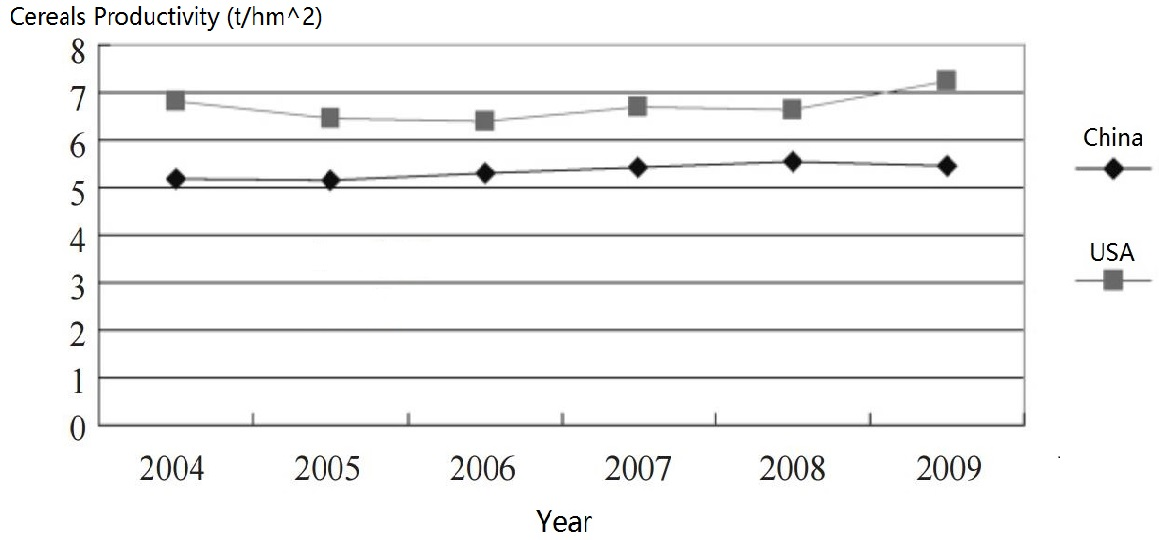
\includegraphics[scale = 0.45]{pics/tperhm.jpg}
\end{center}
\end{table}
\begin{table}[ht!]
\begin{center}
\caption{Labor Dedicated For Agriculture}
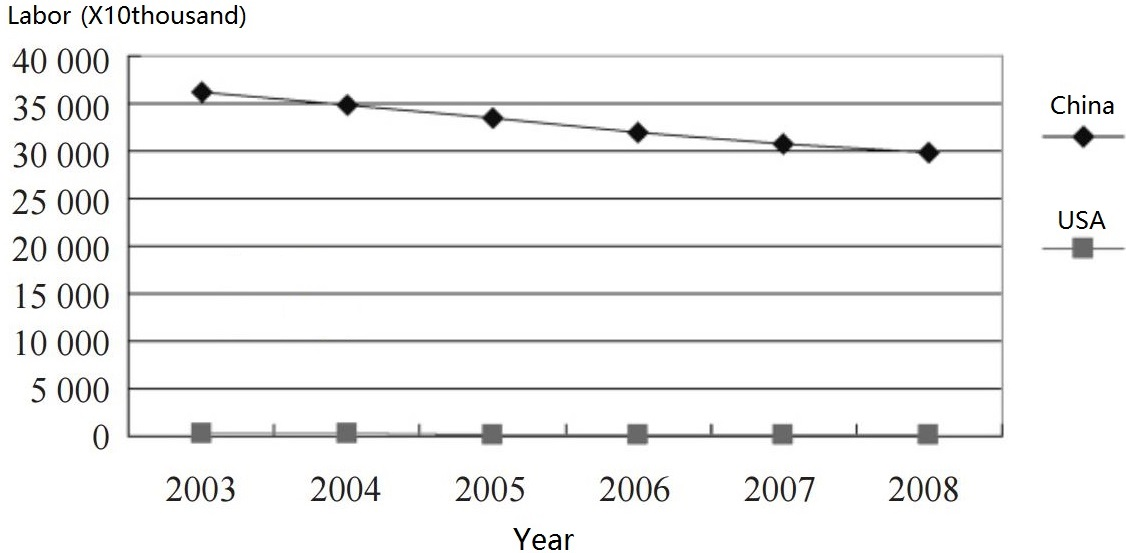
\includegraphics[scale = 0.45]{pics/10k.jpg}
\end{center}
\end{table}
\begin{table}[ht!]
\begin{center}
\caption{Per Capita Arable Land}
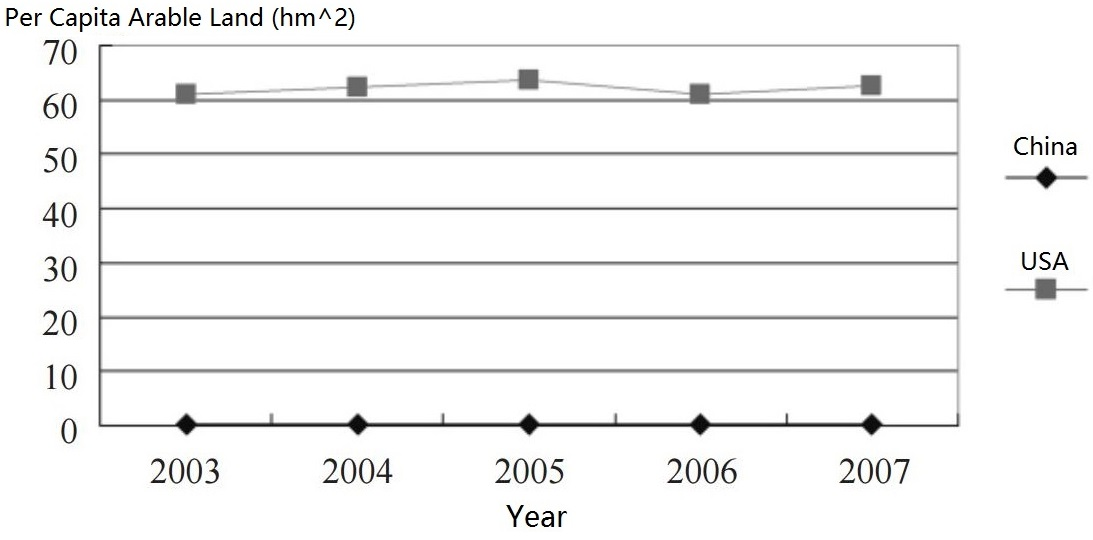
\includegraphics[scale = 0.45]{pics/capitahm2.jpg}
\end{center}
\end{table}
The inefficient productivity and scarcity of arable land brought poverty to Chinese farms. The average net income per capita of Chinese rural family is as low as 7916.6RMB in 2012, which is about 1250USD. \cite{income2012} 

Agriculture in China is dramatically different than in the United States. Although the agricultural structure in China has been modernizing for years, it is still rare to see  modern farm machinery in the field. This situation is caused by two reasons. First, the arable land for each farmer is too small to use big machines, and it is small enough that the traditional ways still work. The second reason is that the annual income for each rural family is too low to buy a big machine. A basic agriculture tractor with 50-75 horsepower is typically from \$20,000 to \$40,000.\cite{tractorcost} And the GPS units cost vary from different systems. Basic WAAS light bars cost about \$2,000 with accuracy from 12 to 15 inches. The RTK GPS units typically cost \$12,000 to \$25,000, plus a \$750 to \$1,500 annual subscription service fee.\cite{PriceR} This is much more than what a Chinese rural family can afford. 



